\documentclass[12pt,a4paper]{article}
\usepackage[utf8]{inputenc}
\usepackage[english]{babel}
\usepackage{setspace}
\usepackage{geometry}
\usepackage{graphicx}

\newgeometry{left=1in, top=1.25in, bottom=1.25in, right=1.5in}

\title{Space Debris Classification}
\author{Daniel Kolosa}
\date{04-18-2017}

\doublespacing

\begin{document}
\maketitle

\section{Introduction}
This project is a study to attempt to create a model to classify a portion of debris orbiting Earth. The first section is an itroduciton describing the backgound material, what is space debris and why is it an issue. The second section describes the dataset that is used for the statistical model. The third section will dicuss the statistical model itself and why it was chosen. The fourth section will look at the results obtained from the model and what conclusions can be drawn from the dataset and the model and the possible future work and implementations of this model.   

\section{Backgoround}
Ever since humans have been sending things into space we have not been cleaning up after ourselves. Sending things into space requires a lot of energy and cost, so bringing things back costs even more. The debris that is in space is the remains of dead satellites, rocket chasis, engines, components of space stations, and other micellaneous items. Fortunatly, some items that are close enough to Earth reenter the atmosphere are burn up on reentry But there are still many objects that will remain in orbit. 

\section{Methods and Data}
Before going into the statistical analysis methods used, it is important to understnad the dataset used for satellite tracking.
The dataset used is a collection of objects orbiting in the Low-Earth orbit (LEO) region. There are many other regions including, geo-synchronous orbit (GEO), high earth orbitl (HEO). Satellite tracking data is encoded in a two line element set. The two line element set encodes position and velocity of a satellite based on its orbital elements. Orbital elements is a coordinate system used to describe the shape of an orbit. The two element set also includes data such as identification number, security classification either classified or unclassified epoch lauch dates, and atmospheric drag coefficients. The position and velocity of the objects are computed using simplified pertubation models. The simplified pertubation models are used to compute the orbital state of an object which taking into account the shape of the Earth, radiation, atmospheric drag, and gravitional influence from the Moon and Sun.

The dataset used for this project is provided by tarck-sat.org. This organization collects and maintains datasets of satelliete position status and position data. The data is obtained from NORAD(North American Aerospace Defense Command) and NASA. The dataset will be analyzed using various methods. One interesting thing to look at is to see which countries have which objects. This is a good insight into what countries have what type of debris. The object type seen in this dataset are: debris, payload, rockect bodies, and others. Debris in this context consists of satellite and spacecraft fragments, payload is made up of capsulues of supplies or satellites. Rocket bodies consist of discarded roackets that were used to launch objects into orbit. 

Along with the object type the radar corss-section is an important metric to look at. The radar cross section is used to estimate the cross-sectional area of an object. For the purposes of this study, a larger radar cross section means that an object is larger. Speciic values for the radar cross section is not provided due to security reasons or lack of accuracy from the ground sttion sensors. Radar cross section is divided into three categories, small, medium, and large. Small are objects <$.1 m^2$, medium are objects between .1$m^2$ and 1$m^2$, and large objects are > $1m^2$.

The given dataset also provides orbital element data. The orbital element data provided are: apogee, perigee, inclination, and Period. The apogee and perigee are the maximum and minimum radii of an eliptical orbit, respectivly. The inclination is the tilt angle of the orbit relative to the Earth's equator and the period is the time it takes for the object to orbit the Earth in one revolution. 

The dataset provided will be used to create a classifier. This classifier will dtermine how much potential risk an object is. This risk metric is a function of two things, the mean orbit spped of an object and the rader cross section. The classifer works by determineg that object with large cross sectional area and high velocities have the most risk of damaging or colliding with other objects then slower and smaller objects.

As menthioned earlier, the risk assesment will be based on the mean obit speed, the mean orbit spped can be determined from the equation below.
\begin{equation}
v = \frac{2a}{T}
\end{equation}
where T is the orbit period given by the dataset in seconds and a is the semimajor axis in kilometers, given in the equation below

\begin{equation}
a = \frac{r_p + r_a }{2}
\end{equation}
Where $r_p$ is perigee and $r_a$ is apogee.



\section{Results}
Creating some plots of the dataset will help with getting an understanding on why there is an issue on debris. The plot shown below shows which countries contribute the most to this dataset. 

In order to build a practical statistical model, it is important to generate plots of the dataset to see the relasionships of the data.
\\
graph here
\\
The plot shows that Russia (CIS), China (PRC), and the United States (US) have launched the most objects into space over the span of the beginning of the space program. 

As mentioned earlier, the dataset provided contains not only debris but also other objects. The figure below shows what kind of objects and how many objects are in each category.
\begin{center}
	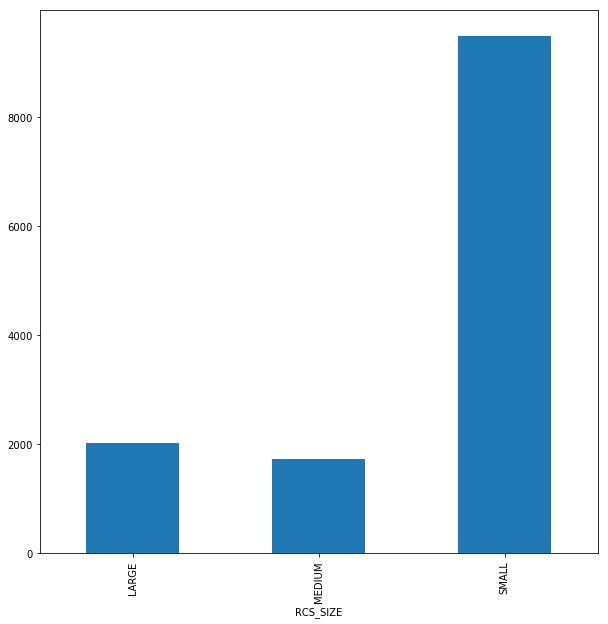
\includegraphics[scale=0.3]{figures/RCS_size.png}
	\captionof{figure}{Distribution of object size}
	\label{fig:RCS_size}
\end{center}
It can be seen from the figure above, that debris make up a significant amount of objects of the dataset. Another interesting plot to look at is the number of objects for the three different sizes.
\begin{center}
	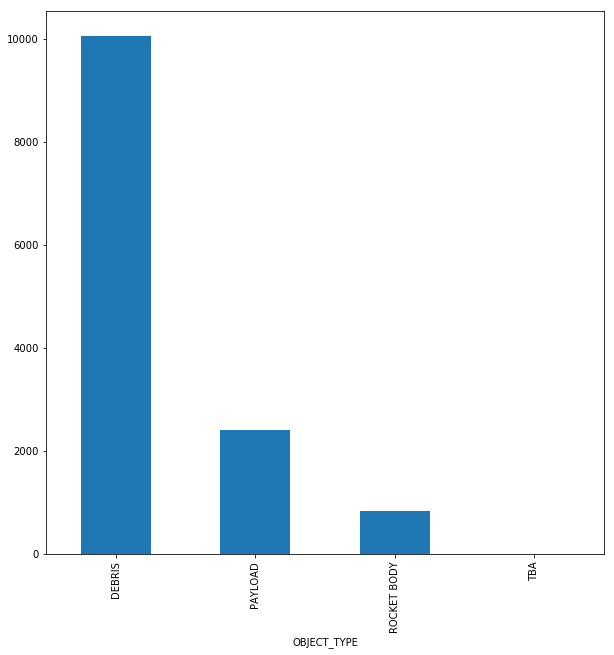
\includegraphics[scale=0.3]{figures/object_types.png}
	\captionof{figure}{Number of objects by object type}
	\label{fig:object_types}
\end{center}
Looing at the plot above it can be seen that the most objects in the dataset have a small cross section. This gives a good visualization of what kind of debris is in orbit. 

Now the statistical model will be looked at. The dataset used was the orbital speed and the radar cross section. The data was split into the training and test data with 80\% being the traiing data and 20\% being the test data. The training data was then fitted to a k-means classfier with 3 clusters. Each cluseter designates the size of the radar cross section, small, medium, and large. The figure below shows a plot displaying the objects in the dataset by cross section and the mean orbit spped.  


\section{Conclusion}
This papaer goes into the background inforamtion on space debris. Then the dataset and approaches were discussed. Then the results of the statistical analysis were discussed.

The future work of this project could include implementing more complicated classification models like using neural networks.
Given the results of this project with the large amount of debris orbiting Earth, many people working on trying to midigate the orbital debris problem. 

 
\end{document}
